\programme{ Gas combustion}
{\huge subroutines: co** and d3p*, ebu*, lwc*, pdf*}

Flames with gaseous fuels can be categorized in premix, diffusion or
partial-premix.


%%%%%%%%%%%%%%%%%%%%%%%%%%%%%%%%%%
%%%%%%%%%%%%%%%%%%%%%%%%%%%%%%%%%%
\section{Premix: Eddy Break Up}
%%%%%%%%%%%%%%%%%%%%%%%%%%%%%%%%%%
%%%%%%%%%%%%%%%%%%%%%%%%%%%%%%%%%%

The original Spalding model \cite{1} was written for a situation where
the whole boiler is full with the same mixture ({\small only one
inlet}) ; the key-word of which is {\em"If it mixes, it burns"}.\\

If the chemistry is fast, vs. mixing, fluid particles are made of
fresh gases or of burned ones. This situation is described by a
progress variable ({\small valued 0 in fresh gases and 1 in burnt
ones}) with a source term: the reaction one. The mixture of totally
fresh or totally burnt gases, called intermittency, leads to a maximal
variance of the progress variable determined by the mean value of the
progress variable.\\
\begin{equation}
C"^{2} max = (Cmoy -Cmin).(Cmax-Cmoy) = Cmoy . (1-Cmoy)
\end{equation}


The mixing of fresh and burnt gases is the dissipation of this
variance and it induces the conversion of fresh gases in burnt
ones. So the source term for the ({\small mean}) progress variable is
the dissipation of its ({\small algebraic}) variance.\\

In \CS the progress variable chosen is the mass fraction of fresh
gases, so:\\
\begin{equation}
S(Ygf) = - Cebu . \rho . \frac{\epsilon}{k} . Ygf . (1-Ygf)
\end{equation}

Where Cebu is a constant, supposedly "universal", fitted around 1.6
({\small only advanced users can adjust this value}).\\


Some improvements have been proposed, and largely used, for situations
with mixture fraction gradient ({\small staggering of reactant(s)})
but are not theorically funded. The simplest extension is available
({\small options 2 and 3 }) in \CS with one extra equation solved for
f the mean of mixture fraction: the corresponding hypothesis is "no
variance for mixture fraction" ... a little bit surprising in an EBU
context ({\small maximal variance for progress variable}). The choice
of the fresh gas mass fraction appears now quite pertinent: the
computation of species mass fraction can be done, with respect to the
mean mixture fraction, both in fresh ({\small the mass fraction of
which is Ygf}) and burnt gases ({\small the mass fraction of which is
(1-Ygf)}).\\
\begin{equation}
Y_{Fuel} = Y_{gf}.f + (1-Y_{gf}) . Max(0 ; \frac{f-fs}{1-fs})
\end{equation}
\begin{equation}
Y_{Ox} = Y_{gf}.(1-f) + (1-Y_{gf}) . Max(0 ; \frac{fs-f}{fs})
\end{equation}
\begin{equation}
Y_{Prod} = (1-Y_{gf}) . Min( \frac{f}{fs} ; \frac{1-f}{1-fs} )
\end{equation}
Where fs is the stoechiometric mixture fraction.\\

In adiabatic conditions the specific enthalpy of gases ({\small in
every combustion model the considered enthalpy contains formation one
and heat content, but no terms for velocity or pressure}) is directly
related to the mixture fraction ({\small as long as the inlet
temperature for air and fuel is known}). When heat losses, like
radiation, are taken in account, an equation has to be solved for the
mean enthalpy ({\small such an equation is needed so when some entries
have different temperatures -partial preheat- enthalpy is then used as
an extra passive scalar}). In industrial processes, the aim is often
to transfer the heat from burnt gases to wall ; even for heat loss the
wall temperature is near to fresh gases temperature and the main heat
flux takes place between burnt gases and wall. So in \CS the specific
enthalpy of the fresh gases is supposed to be related to mixture
fraction and the specific enthalpy of burnt gases is locally computed
to reach the mean specific enthalpy. This way every heat loss removed
from the mean enthalpy is "paid" by the hottest gases.\\

\begin{equation}
hmean = Ygf.hgf(f) + (1-Ygf).hbg => hbg
= \frac{hmean-Ygf.hgf(f)}{1-Ygf}
\end{equation}

Where f ({\small in hgf(f)}) is the local mean of the mixture fraction
or a constant value ({\small in regular EBU model}).

%%%%%%%%%%%%%%%%%%%%%%%%%%%%%%%%%%
%%%%%%%%%%%%%%%%%%%%%%%%%%%%%%%%%%
\section{Diffusion: PDF with 3 points chemistry}
%%%%%%%%%%%%%%%%%%%%%%%%%%%%%%%%%%
%%%%%%%%%%%%%%%%%%%%%%%%%%%%%%%%%%

In diffusion model, the combustion is supposed limited only by mixing
({\small between air and fuel}), so the reaction is assumed to reach
instantaneously its equilibrium state and the temperature and
concentrations can be computed for every value of the mixture
fraction. In \CS the implemented version uses an extra hypothesis:
the reaction is complete ; so if the mixture is stoechiometric, the
burnt gases contains only final products ({\small none unburnt like
CO...}). As a consequence, every concentration is a piecewise linear
function of the mixture fraction (subroutines: \fort{D3PPHY, D3PINT,
CPCYM,FUCYM}) .\\
\begin{equation}
0<f<fs => Yi(f) = Yair + \frac{f}{fs} . (Ys-Yair)
\end{equation}
\begin{equation}
fs<f<1 => Yi(f) = Ys + \frac{f-fs}{1-fs} . (Yfuel-Ys)
\end{equation}\\
\begin{figure}[h]
%\centerline{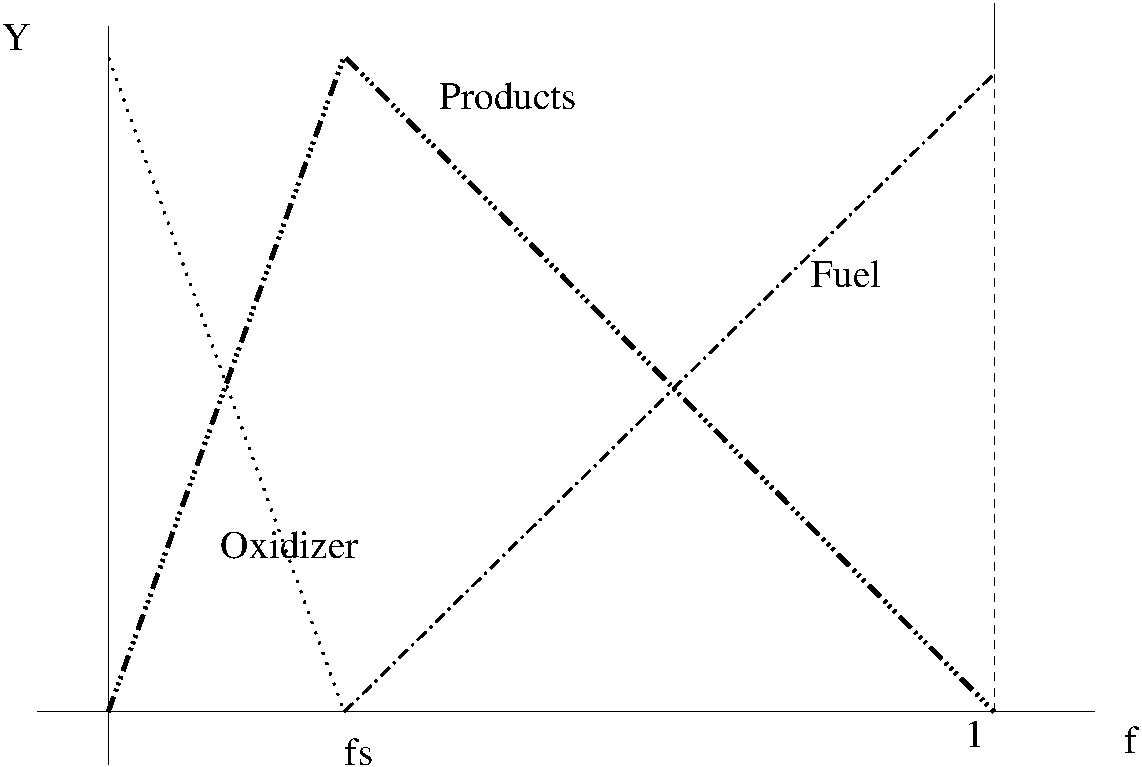
\includegraphics[height=3cm]{../Comb/Cogz/Images/Yf.pdf}}
\caption{mass fraction of global species are piecewise linear with mixture fraction}
\end{figure}
Where fs is the stoechiometric mixture fraction, Yair and Yfuel are
concentrations in ({\small supposed unable to react: inert}) initial
reactant, Ys concentrations in products of the complete reaction of a
stoechiometric mixture ({\small in such products, the chemical
reaction is no more possible: inert}).\\

The diffusion model uses two equations for the mixture fraction and
its variance both of them having no reaction term. The mean and the
variance of the mixture fraction are used to presume the Probability
Density Function for the mixture fraction. In \CS the shape proposed
by Borghi \cite{4} with a rectangle and Dirac's peak is used
(subroutines \fort{COPDF, CPPDF, FUPDF}).\\

\begin{figure}[h]
%\centerline{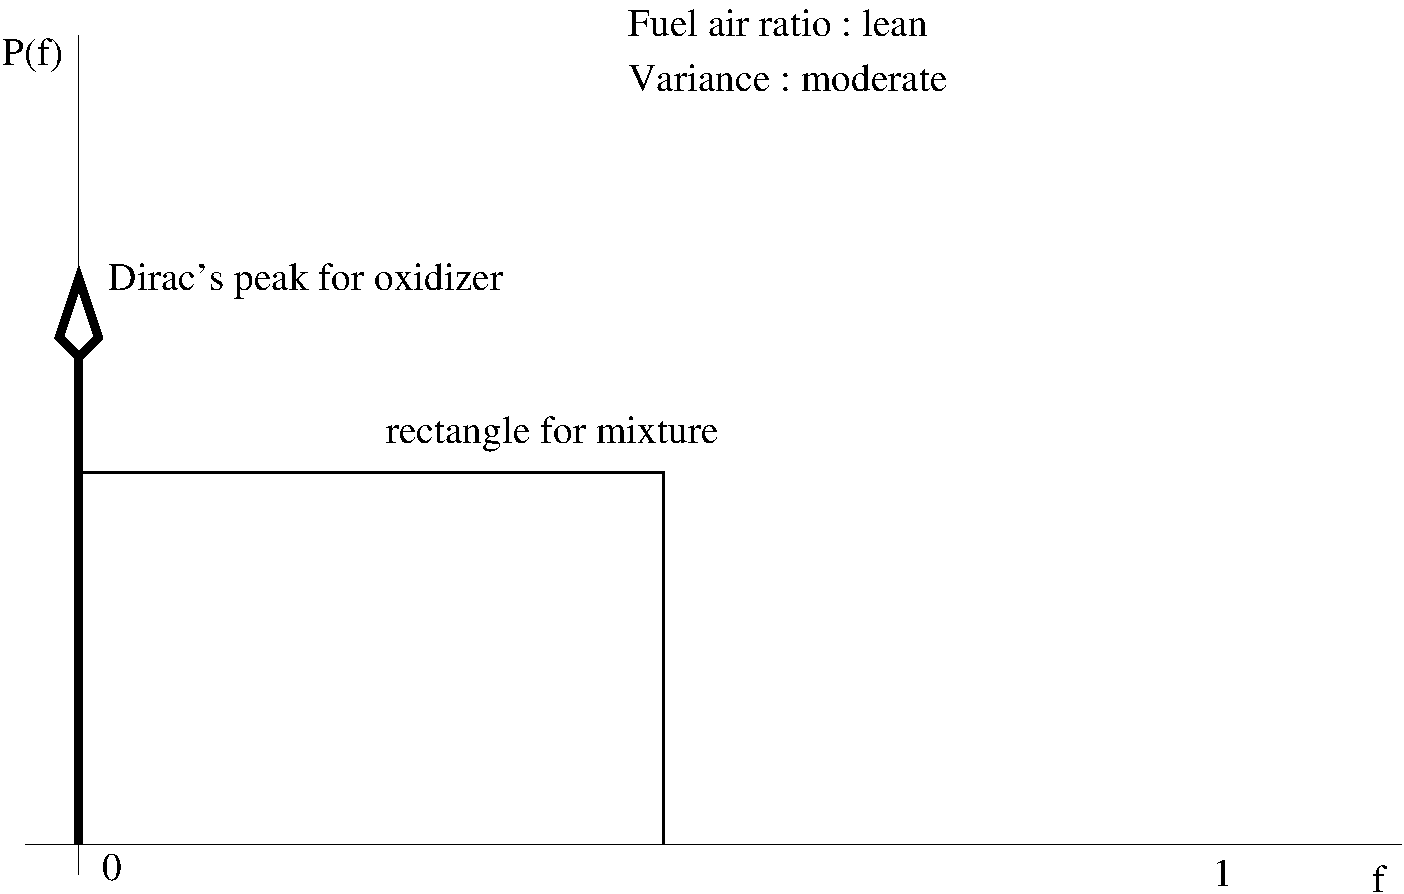
\includegraphics[height=4cm]{../Comb/Cogz/Images/Pf.pdf}}
%\centerline{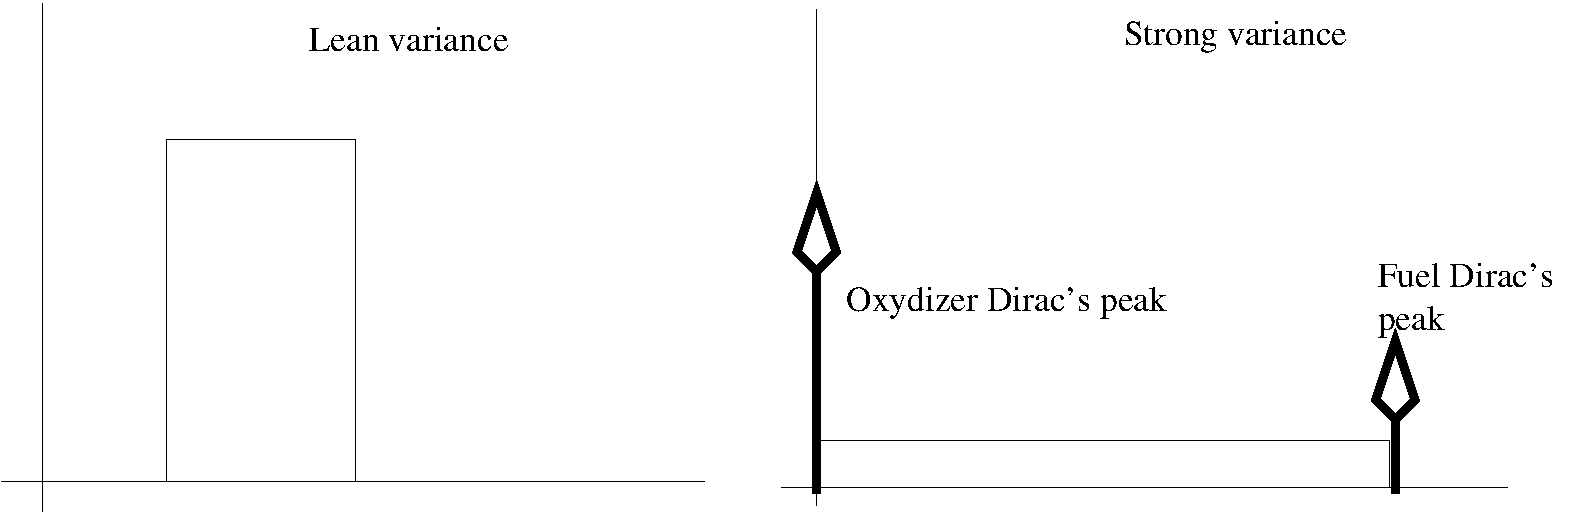
\includegraphics[height=2.5cm]{../Comb/Cogz/Images/Pf2.pdf}}
\caption{Examples of presumed PDF: cheapest form}
\end{figure}
The determination of mean concentration is done by integration the
local concentration weighted by the probability density function. As a
matter of fact, integrate the product of a piecewise linear function
by a constant ({\small height of the rectangle}) is a very simple
exercise: analytic solution are available ({\small the original
Borghi formulation \cite{3} wich uses $\beta$ function was much more
computationaly expensive}).

In adiabatic condition, the specific enthalpy of the mixture is a
linear function of the mixture fraction ({\small the enthalpy is not
modified by the reaction}). As for premix combustion, an assumption is
done "the hotter the gases, the worse the heat losses", so the
enthalpy of pure oxidiser and fuel are supposed not to be modified in
permeatic conditions, the enthalpy of products hs ({\small at the
stoechimodtric mixture fraction}) is an unknown or auxiliary
variable. The enthalpy of the mixture is supposed linear piecewise
with f ({\small like concentrations but with an unkwnon at fs}) and
the resulting mean enthalpy ({\small weighted by PDF}is linear in
hs. Fitting with the equation for the mean enthalpy ({\small wich
takes in account radiation and other heat fluxes}), hs is determined
and, consequently the temperature at fs and the mean temperature can
be computed.

\begin{figure}[h]
%\centerline{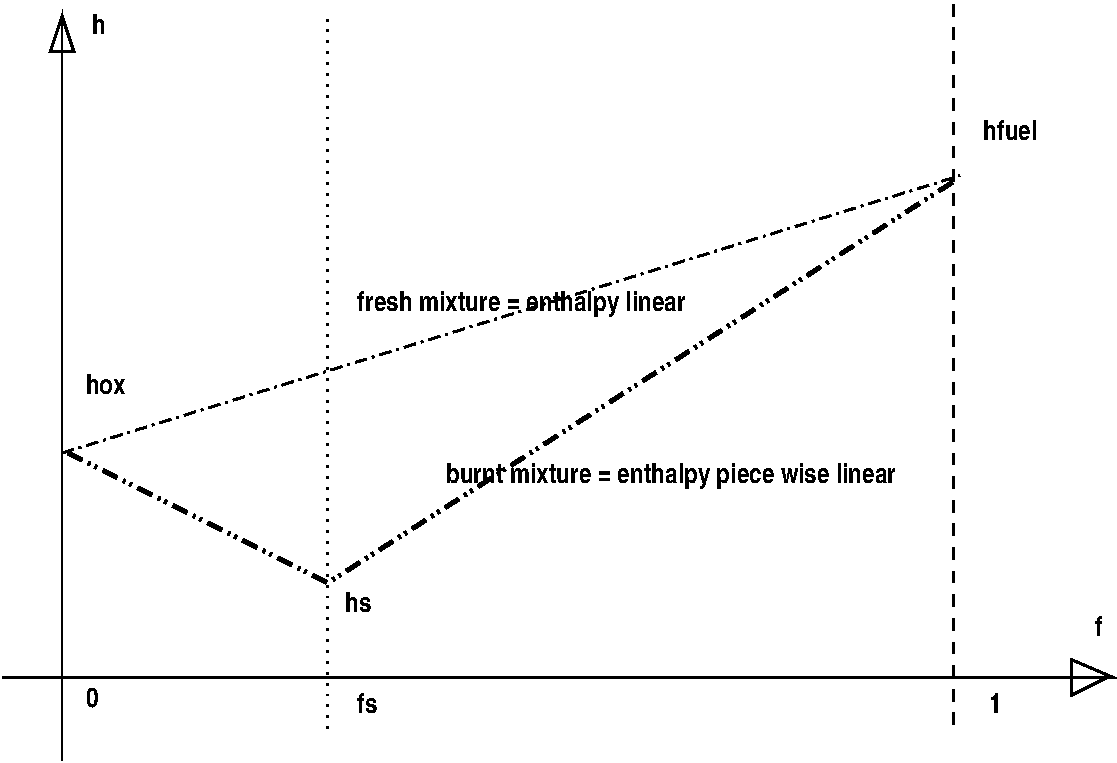
\includegraphics[height=4cm]{../Comb/Cogz/Images/hf.pdf}}
\caption{Enthalpy of products is determined to account for heat losses }
\end{figure}

%%%%%%%%%%%%%%%%%%%%%%%%%%%%%%%%%%
%%%%%%%%%%%%%%%%%%%%%%%%%%%%%%%%%%
\section{Partial premix: Libby Williams models}
%%%%%%%%%%%%%%%%%%%%%%%%%%%%%%%%%%
%%%%%%%%%%%%%%%%%%%%%%%%%%%%%%%%%%


\CS has been the test-bed for some versions of Libby-Williams model \cite{2}, like inplemented then incremented by Ribert \cite{5} and Robin \cite{6}.

The Libby \& Williams model have been developped to address the
description of the combustor can of gas turbine in regime allowing a
reduction of NOx production using ({\small sometimes very}) lean
premix: by this way, the combustion occurs at moderate temperatures
avoiding the hot spots which are favourable to thermal NOx
production. As a consequence of the moderate temperatures, the
chemistry is no more so fast and the stability is questionnable. To
ensure it a diffusion flame called pilot takes place in the center of
the combustor. So, if the main flow is premixed, both pure fuel and
pure oxidiser are introduced in the combsutor leading to continuous
variation of the equivalence ratio ({\small always the mixture
fraction}). This situation is clearly out of the range of both EBU and
PDF models, moreover the limitation by the chemistry is needed
({\small for stability studies}).\\

Originally, Libby \& Williams proposed a presumed PDF made of two
Dirac's peak, Ribert showed that this PDF can be determined with only
the mean and the variance of the mixture fraction and a reactive
variable ({\small by now, the mass fraction of fuel is used}). Then
some undeterminations seem awkward and Robin \& al. propose a four
Dirac's peak PDF whose parameters are determined with the same
variables and the solved ({\small transported}) covariance ({\small of
the reactive variable and the mixture fraction}) as an extra solved
field. With the condition corresponding to every Dirac's peak a global
chemistry description is used ({\small source term for every variables
is a weighting of the reaction fluxes}).\\ With two peaks
distribution, the two-variable PDF is restricted to one line, crossing
the mean state and the slope of which is the ratio of variances
({\small chose of the sign is user free, ... but relevant: expertise
is needed}). The correlation between variables is unity.\\ On this
line the distribution is supposed to obey a modified Curl
model \cite{7}.\\
\begin{figure}[h]
%\centerline{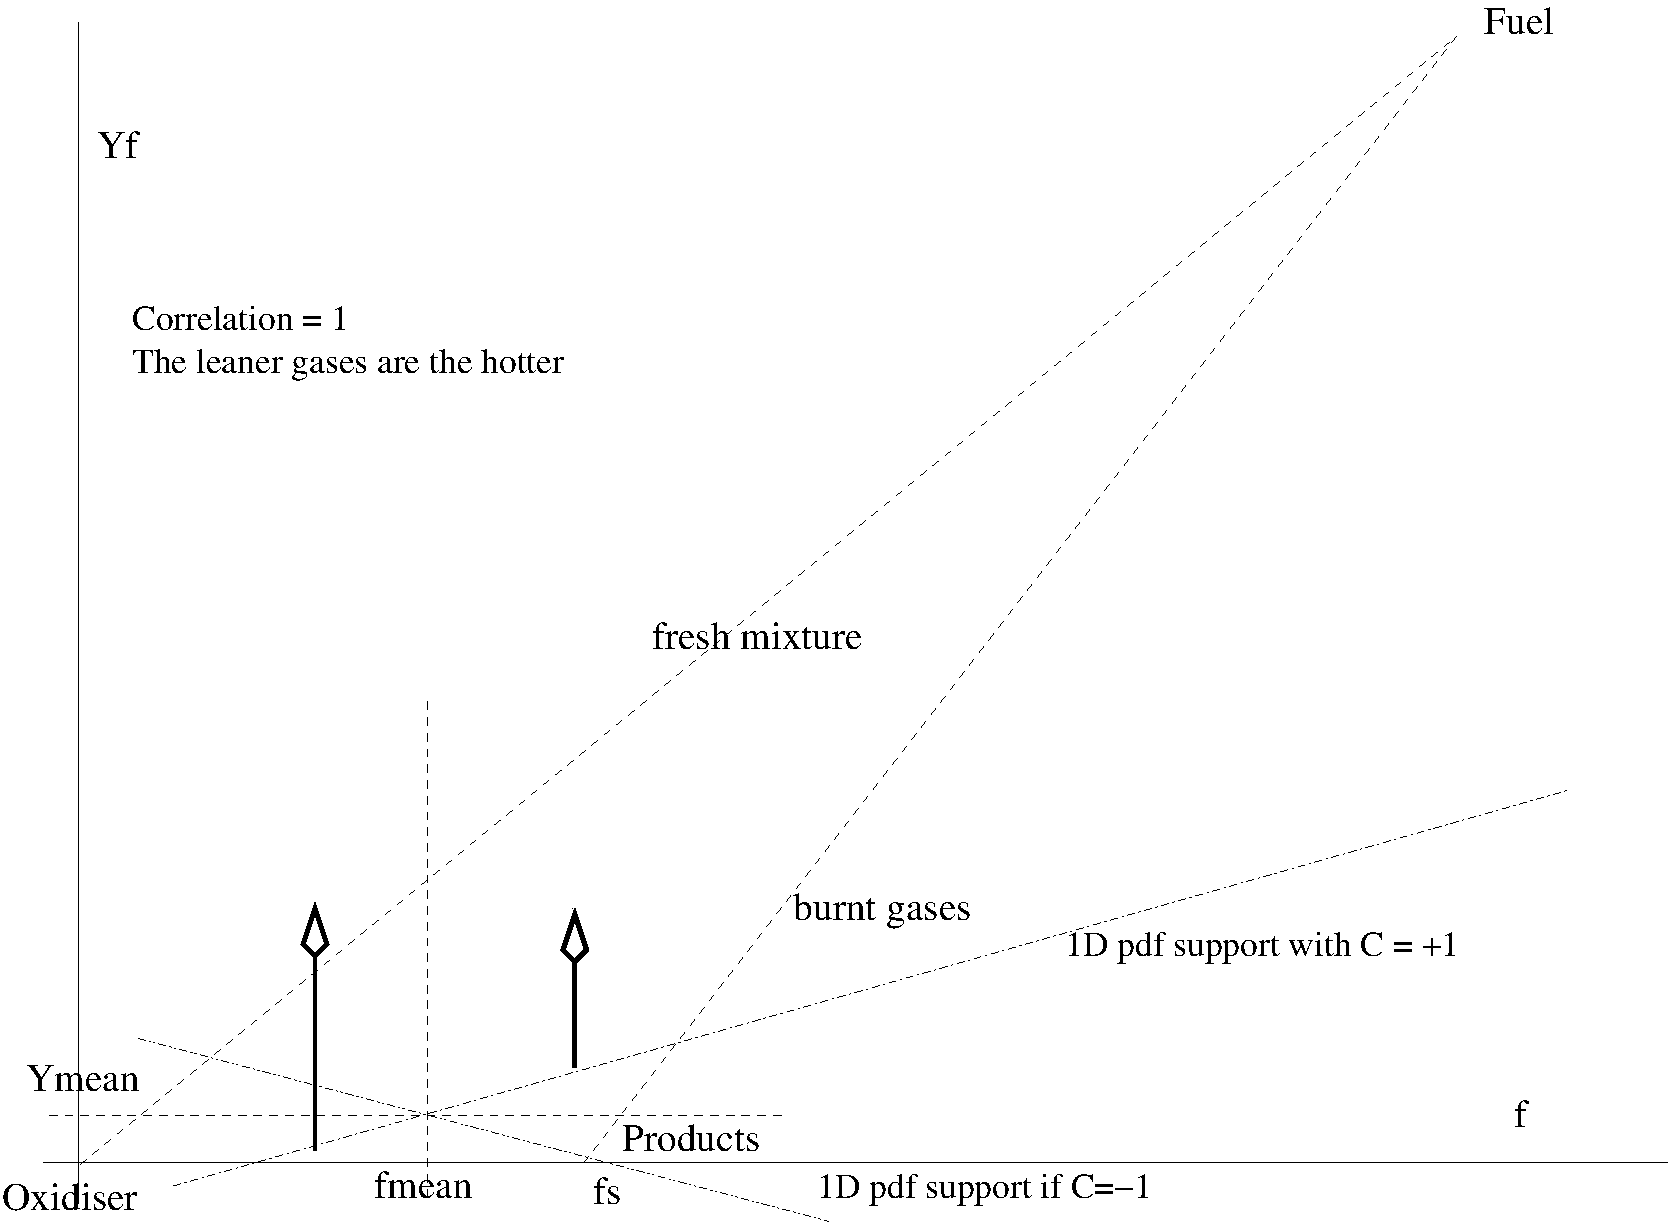
\includegraphics[height=5cm]{../Comb/Cogz/Images/LW2.pdf}}
\caption{PDF recommended by Libby \& Williams: still undetermined}
\end{figure}
With three or four peaks distribution, the whole concentration space
is available and the determination of the covariance allows evolution
of the correlation ({\small with f and Yf, it have been shown that the
correlation is positive in mixing layer and can become negative across
flame: the particle nearer of stoechiometry being able to burn -then
destroy Yf- faster than poor ones}). \\
\begin{figure}[h]
%\centerline{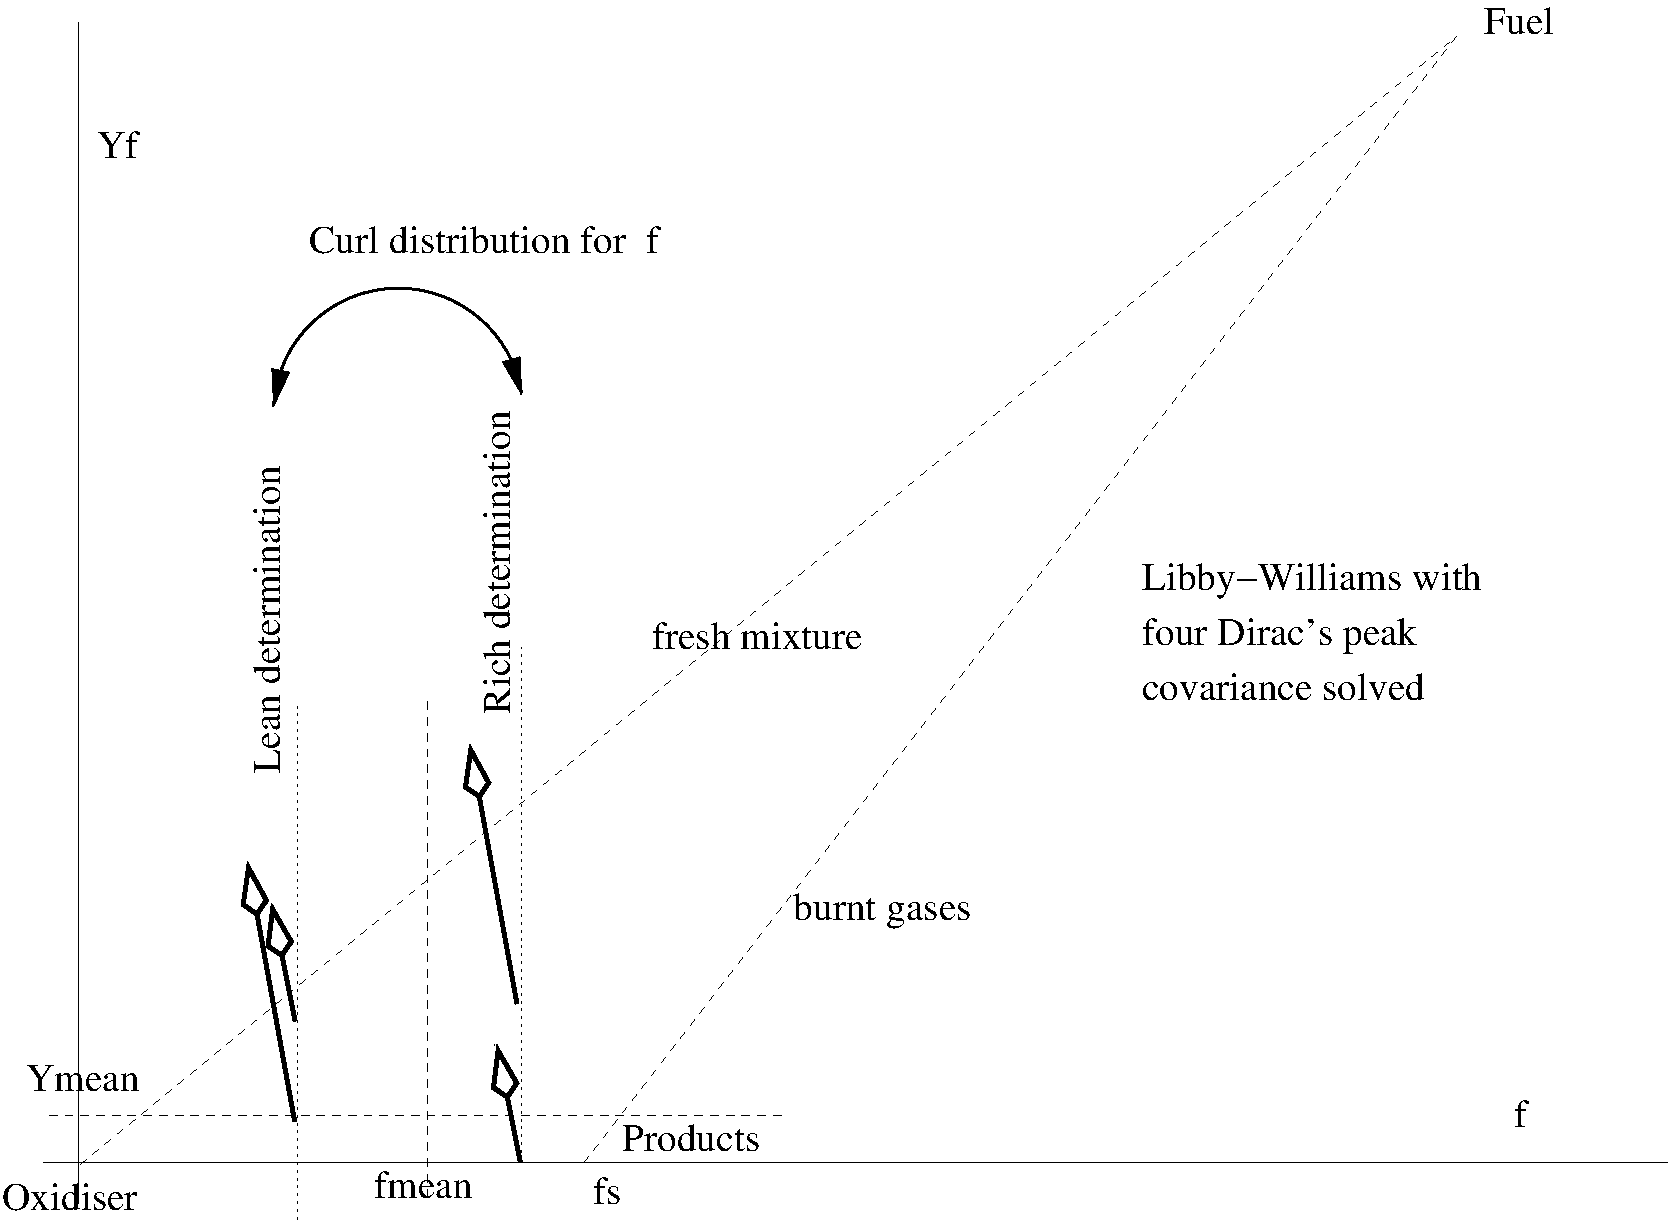
\includegraphics[height=5cm]{../Comb/Cogz/Images/LW4.pdf}}
\caption{PDF form in LWP approach: succesive modified Curl distributions}
\end{figure}
In adiabatic conditions, the temperature can be computed for every
pair (f,Yfuel), allowing the determination of the kinetic constant.\\
As previously, with heat losses, it is assumed that the hottest gases
have lost the more, the enthalpy of the products at stoechiometric
point (fs,0) is an auxiliary variable, the enthaply being considered
as a piecewise bilinear function. Fitting mean transported enthalpy
and integrated ones, allows to determine the enthalpy of
stoechiometric products, then the enthalpy and temperature in the
peaks conditions and, ({\em in fine}) the reactions fluxes.




%==================================
%==================================
\section{Bibliography}
%==================================
%==================================
\begin{thebibliography}{7}

\bibitem{1}
{\sc Spalding, D.B., {\em et al.}},\\
{\em Mixing and chemical reaction in steady confined turbulent turbulent flames},\\
13th Int.Symp. on Combustion , pp. 649-657, (1971).

\bibitem{2}
{\sc Borghi, R. {\em et } Moreau, P.},\\
{\em Turbulent combustion in a premixed flow},\\
Acta Astronautica, 4, pp. 321-341, (1977)

\bibitem{3}
{\sc Borghi, R. {\em et } Dutoya, D.},\\
{\em On the scale of the fluctuation in turbulent combustion},\\
17th Int.Symp. on Combustion, (1978).

\bibitem{4}
{\sc Libby, P.A. {\em et } Willimas, F.A.},\\
{\em A presumed PDF analysis of lean partially premixed turbulent combustion},\\
Comb. Sci. Technol., 161 , pp. 351-390, (2000).

\bibitem{5}
{\sc Ribert, G. {\em et al.}},\\
{\em Modeling turbulent reactive flows with variable equivalence ratio: application to the calculation of a reactive shear layer},\\
Comb. Sci. Technol., 176 , pp. 907-923, (2004).

\bibitem{6}
{\sc Robin, V. {\em et al.}},\\
{\em Relevance of approximated PDF shapes for turbulent combustion modeling with variable equivalence ratio},\\
ICDERS, (2005) to be published.

\bibitem{7}
{\sc Curl, R.L.},\\
{\em Dispersed phase mixing: theory and effects in simple reactors},\\
AIChE J., 9 , pp. 175-181 (1963).




\end{thebibliography}
\newpage
%%%%%%%%%%%%%%%%%%%%%%%%%%%%%%%%%%
%%%%%%%%%%%%%%%%%%%%%%%%%%%%%%%%%%
\section{Discretisation}
%%%%%%%%%%%%%%%%%%%%%%%%%%%%%%%%%%
%%%%%%%%%%%%%%%%%%%%%%%%%%%%%%%%%%

Some applied mathematics are involved in pdf parameters determination
({\small rectangle and modified Curl}) and for integration ({\small
species mass fraction, temperature, density and so on}).\\

%%%%%%%%%%%%%%%%%%%%%%%%%%%%%%%%%%
%%%%%%%%%%%%%%%%%%%%%%%%%%%%%%%%%%
\subsection{Rectangle and Dirac's peaks probability density function}
%%%%%%%%%%%%%%%%%%%%%%%%%%%%%%%%%%
%%%%%%%%%%%%%%%%%%%%%%%%%%%%%%%%%%

This type of pdf is used in diffusion flames both for gas combustion
or dispersed fuel ones ({\small coal and heavy fuel oil}). In gas
mixture, the pdf is build for an equivalence ratio for fuel ({\small
inert scalar variable}) ranging on [0, 1]. For disperse fuel, due to
vaporisation, or pyrolysis, and heterogeneous combustion two or three
gaseous fuels are taken in account, each of them having its own inert
scalar, so the PDF is build for an inert scalar incoming with air and
ranging from a minimum value and one ; the minimum value for air
tracker is due to heterogeneous combustion: some air is needed to
allow heterogeneous combsution and carbon releasing ({\small as carbon
monoxide}) ; after some heteregenous reaction took place, air is
lacking for gas combustion ({\small at the bottom stone mile of the
range allowed for the inert scalar associated with air, oxygen
concentration is zero valued}). The algorithm for pdf parameters
determination, can be wrotten in a general form on every variable's
range.\\

If the allowed range for the variable is [$f_{min} ; f_{max}$],
knowing the mean and variance of the variable allow to determine first
the shape ({\small alone rectangle, rectangle and one Dirac's peak at
one boundary, two Dirac's peak at boundaries and rectangle}) and then
the three pertinent parameters ({\small three conditions given by
momenta $m_{0}=1, m_{1}=mean, m_{2}=mean^{2}+variance$}).\\

- for a lonesome rectangle Dirac's peak intensity is null, the three
  parameters are: the begin and end values of the rectangle and its
  heigth\\

- for a rectangle with a Dirac's peak at one boundary ({\small which
  is determined during the choose of shape}), one of the rectangle
  hedge is fixed at this boundary, so the three parameters are: the
  other rectangle hedge, height of rectangle, intensity of the Dirac's
  peak\\

- for a two Dirac's peak distribution, both rectangle hedges are at
   the boudaries, so the parameters are the rectangle height and the
   Dirac's peak intensity.\\

Quite complicated tests ({\small computationnaly expensive}) can be
done to determine only the relevant parameters, and therefore spare
computations, or general computaions of parameters can be done and
afterwards tested ({\small if rectangle too large then attempt with
one Dirac's peak. If too large again then two peaks would be
convenient}).
 
 

%%%%%%%%%%%%%%%%%%%%%%%%%%%%%%%%%%
%%%%%%%%%%%%%%%%%%%%%%%%%%%%%%%%%%
\subsection{Composition in total turbulent reaction assumption}
%%%%%%%%%%%%%%%%%%%%%%%%%%%%%%%%%%
%%%%%%%%%%%%%%%%%%%%%%%%%%%%%%%%%%

With the above Probability Density Function and assumption of
concentrations piecewise linear vs. the variable, it is quite easy to
integrate and found the mean concentrations. For gas diffusion flame
this is done by \fort{D3PPHY, D3PINT}, it seems more relevant to
explain the algorithm in a more complicated case: for heavy fuel
oil \fort{FYUCYM} or for coal \fort{CPCYM} three reactions are
considered. \\

- Coal is assumed to undergoes two competitve pyrolysis reactions, the
  first releasing organic compound summarized as $CH_{x1}$, the second
  releasing $CH_{x2}$ ({\small with $x1 > x2$}), both of them
  releasing $CO$. Then the heterogeneous combustion of char release
  $CO$. So three reactions are supposed to succed ({\small both in
  time and in priority to access to oxygen}). First of all partial
  dehydrogenation ({\small lowering saturation}) of $CH_{x1}$ to
  produce water vapor and $CH_{x2}$. Then the $CH_{x2}$ ({\small
  produced by pyrolisis or by $CH_{x1}$ partial oxydation}) is
  converted to water vapor and carbon monoxide. Last, carbon monoxide
  $CO$ is converted to carbon dioxide $CO_{2}$.\\

- Heavy fuel oil is supposed to undergoes a progressive evaporation,
  releasing a fuel vapor $CH_{x}$, $CO$, $H_{2}S$ and a char
  particle. Then heterogenous oxidation of char releases $CO$. Three
  reactions are supposed to succeed. First, the conversion of $CH_{x}$
  to water vapor and $CO$. Then the oxidation of $H_{2}S$ to water
  vapor and $SO_{2}$. Last, carbon monoxide is fully oxidised.\\

Both for coal and heavy fuel oil, the assumption of a diffusion
flamelet surrounding particles is done. All of the reducing gases are
supposed mixed ({\small to constitue a local mean fuel}) and the
diffusion flammelet take place between this mixture and pure oxidiser
({\small but for solid particles introduced wet, when a first drying
process releases water vapor which is mixed with air}) and the
composition is described with respect to the inert scalar introduced
with air: \fort{f4}.\\

For the description of compositions ({\small as piecewise linear
functions}) the composition is computed in some remarkable points:
the local mean fuel \fort{CL}, the oxidiser \fort{F4} and the three
mixture ratio corresponding to the stoechiometry of the three
successive reactions.\\ Before reaction between gases, only exist
species coming from entries or interfacial source term:\\
\begin{figure}[h]
%\centerline{\includegraphics[height=6cm]{../Comb/Cogz/Images/YF0f.pdf}}
\caption{Heavy Fuel Oil before any gas combustion} 
\end{figure}
{\centerline {\em Caution: axis for f4 is reverted, so fuel is on the
right side like in a scheme with a mixture fraction direct axis}}}\\

The oxygen and the hydrocarbon vapor have concentrations linear in f4
on [CL, 1], as long as the stoechiometry of the reaction is known, a
simple equation allows to determine f4s1 the stoechiometric point for
the first reaction ({\small where both oxygen and hydrocarbon
vanish}).  The first reaction is the conversion of some hydrocarbon
vapor to carbon monixide and water vapor ({\small not plotted in an
optimistic attempt to lighten the sketch}).\\
\\
\centerline{$CH_{x} + \frac{2+x}{4} O_{2} => CO + \frac{x}{2} H_{2}O $}\\
\\
\begin{figure}[h!]
%\centerline{\includegraphics[height=6cm]{../Comb/Cogz/Images/YF1f.pdf}}
\caption{Heavy Fuel Oil after hydrocarbon conversion}
\end{figure}
\\
Then the rich area can't undergo any reaction ({\small no oxygen
available}) if the PDF(f4) is not zero before F4s1, then some $CH_{x}$
is unburnt.\\

Some $H_{2}S$ can be converted to $SO_{2}$, the carbon monoxide
existing between F4cl and F4s2 is protected from oxidation ({\small
the two first reactions have destroyed free oxygen}). Like previously,
oxygen and hydrogen sulphide have concentrations linear in f4 on
[f4s1, 1] as long as the stoechiometry of the reaction is known, a
simple equation allows to determine f4s2 the stoechiometric point for
the second reaction ({\small where both oxygen and hydrogen sulphide
vanish}).\\
\\
\centerline{$H_{2}S + \frac{3}{2} O_{2} => SO_{2} + H_{2}O $ }\\
\\
\begin{figure}[h!]
%\centerline{\includegraphics[height=6cm]{../Comb/Cogz/Images/YF2f.pdf}}
\caption{Heavy Fuel Oil after H2S oxidation}
\end{figure}
\\
Now oxygen and carbon monoxide have concentrations linear in f4 on
[f4s2, 1], and f4s3 ({\small the point wher the whole oxygne and
carbon monoxide are converted to carbon dioxide}) is easy to
compute.\\
\\
\centerline{$CO + \frac{1}{2} O_{2} => CO_{2} $ }\\
\\
\begin{figure}[h!]
%\centerline{\includegraphics[height=6cm]{../Comb/Cogz/Images/YF3f.pdf}}
\caption{Heavy Fuel Oil after final carbon oxidation}
\end{figure}
\\
To have not any unburnt, the PDF may be zero valued for F4 $<$ F4s3:
every gas particle may have an F4 greater than F4s3.\\

During pulverised coal combustion, two kinds of volatile matters are
considered and the sketch of concentrations during the three
successive reactions is quite similar.\\

The first reaction is a partial dehydrogenation of the light volatile
$CH_{x1}$ to form the species caracteristic of heavy volatile
$CH_{x2}$: in f4s1, all of $CH_{x1}$ ({\small issued from the low
temperature pyrolisis reaction}) is converted, and the $CH_{x2}$
({\small issued from the high temperature pyrolisis reaction}) is
incremented.\\
\\
\centerline{$CH_{x1} + \frac{x1-x2}{4} O_{2} => CH_{x2} + \frac{x1-x2}{2} H_{2}O $}\\
\\
The second reaction is the conversion of this unsaturated hydrocarbon
to carbon monoxide and water.\\
\\
\centerline{$CH_{x2} + \frac{2+x2}{4} O_{2} => CO + \frac{x2}{2} H_{2}O $}\\
\\
And the last ({\small not the least from an energetic point of view})
is the same final oxidation of carbon monoxide to carbon dioxide.\\
\\
Comparisons of the PDF rectangle hedges [$f_{deb} , f_{fin}$] and
remarkable composition points [CL, f4s1, f4s2, f4s3, F4] allows a
simple integration: 1) Dirac's peak intensity are used to weight
composition at boundaries, 2) the piece linear part is integrated with
analytical formulae on each band:\\
\begin{enumerate}
\item rich range, here exists species with the higher calorific value: $CH_{x}$ ({\small in fuel case}) or $CH_{x2}$ ({\small in coal case }):\\  \centerline{[Max($f_{deb}$,CL) ; Min($f_{fin}$,f4s1)]}\\
\item middle-class range $H_{2}S$ or $CH_{x1}$ conversion:\\
 \centerline{[Max($f_{deb}$ , f4s1 ); Min ($f_{fin}$ , f4s2 )]}\\
\item working range, carbon monoxide consumption frees enthalpy:\\ \centerline{ [Max($f_{deb}$ ,f4s2 ); Min ($f_{fin}$ , f4s3 )]}\\
\item poor range, only products and oxidisers:\\ \centerline{ [Max($f_{deb}$ , f4s3 ); Min ($f_{fin}$ , 1)]}\\
\end{enumerate}

For each band (eg. [f4si , f4sj]) concentrations can be written:\\
\centerline{$Ye = Ye(f4si) + \frac{f4-f4si}{f4sj-f4si} . \left( Ye(f4sj)-Ye(f4si) \right) $}\\ 
Integration on the band [b1 , b2] ({\small obviously b1$\geq$f4si \&
b2$\leq$f4sj}) gives the increment:\\
\centerline{$Ye:= Ye + h_{rec}.(b2-b1) + \left[ \frac{Ye(f4si).f4sj-Ye(f4sj).f4si}{f4sj-f4si}+\frac{Ye(f4sj)-Ye(f4si)}{f4sj-f4si}.\frac{b1+b2}{2} \right] $}\\
Where $h_{rec}$ is the height of the PDF's rectangle. 

 
 

%%%%%%%%%%%%%%%%%%%%%%%%%%%%%%%%%%
%%%%%%%%%%%%%%%%%%%%%%%%%%%%%%%%%%
\subsection{Composition in partial turbulent reaction assumption for CO}
%%%%%%%%%%%%%%%%%%%%%%%%%%%%%%%%%%
%%%%%%%%%%%%%%%%%%%%%%%%%%%%%%%%%%

If the final oxidation of carbon monoxide, can't be assumed fast in
respect to mixing ; the main limitation in the kinetic one. So the
above process of concentrations determination is stopped after the two
first reactions ; the resulting, high, content in carbon monoxide
({\small and oxygen}) is the molar sum of both carbon monoxide and
carbon dioxyde. With an extra budget equation for carbon dioxide, the
effective concentrations of carbon monoxide ({\small difference
between "turbulent" integration and transported "already" consumed }),
oxygen and carbon dioxide can be computed, then a reactive source term
for oxidation ({\small of carbon monoxide}) and dissociation ({\small
of carbon dioxide}).

\newpage




